\documentclass[11pt]{article}
\linespread{1}

\renewcommand{\thefootnote}{\fnsymbol{footnote}}

\usepackage{geometry} % see geometry.pdf on how to lay out the page. There's lots.
\usepackage[utf8]{inputenc}
\usepackage[T1]{fontenc}
\usepackage{array}
\usepackage{amsmath,amssymb,latexsym,epic,eepic,epsfig,graphics,psfrag}
\usepackage{amsfonts}
\usepackage{graphicx,float}
\usepackage{color}
\definecolor{mygray}{RGB}{244,244,244}
\definecolor{gray}{gray}{0.5}
\definecolor{myredish}{RGB}{193,33,97}
\definecolor{grayblue}{RGB}{91,112,142}
\definecolor{myorange}{RGB}{255,134,0}
\definecolor{green}{rgb}{0,0.4,0}

\usepackage[english]{babel}

\usepackage[bottom]{footmisc}

\usepackage{fancyhdr}
\pagestyle{fancy}
\lhead{\small\textit{02417 Time Series Analysis - Fall 2011 - Anders Hørsted (s082382)}}
\rhead{\thepage}
\chead{}
\lfoot{}\cfoot{}\rfoot{}

\usepackage{pstricks}
\usepackage{pst-node}
\usepackage{wrapfig}
\usepackage{caption}
\usepackage{multirow}
%\usepackage{fouriernc}
%\usepackage[charter]{mathdesign}
\usepackage{lmodern}
\usepackage[normalem]{ulem}
\geometry{a4paper} % or letter or a5paper or ... etc
% \geometry{landscape} % rotated page geometry

\usepackage{url}


\makeatletter
\renewcommand*\env@matrix[1][*\c@MaxMatrixCols c]{%
  \hskip -\arraycolsep
  \let\@ifnextchar\new@ifnextchar
  \array{#1}}
\makeatother

\newcommand\myimp{\quad\Leftrightarrow\quad}
\newcommand\half{\frac{1}{2}}
\newcommand\myvec[1]{\mathbf{#1}}
\newcommand\mymod[1]{\ (\text{mod }#1)}
\newcommand\myreal{\mathbb{R}}
\newcommand\mynatural{\mathbb{N}}
\newcommand\myinteger{\mathbb{Z}}
\newcommand\mycomplex{\mathbb{C}}
\newcommand\myint{\text{int}}
\newcommand\norm[1]{||\,#1\,||}
\newcommand\bignorm[1]{\big|\big|\,#1\,\big|\big|}
\newcommand\seq[1]{\big\{#1\big\}}
\newcommand\smallseq[1]{\{#1\}}
\newcommand\smallseqtoinf[1]{\smallseq{#1}_{k=1}^\infty}
\newcommand\lonew{\ell^1_w}
\newcommand\lone{\ell^1}
\newcommand\ltwo{\ell^2(\mynatural)}
\newcommand\ip[2]{\langle#1,#2\rangle}
\newcommand\hilbert[1]{\mathcal{#1}}
\newcommand\uinf{u_{\infty}}
\newcommand\erf{\text{erf\,}}
\newcommand\infint{\int_{\infty}^{\infty}}
\newcommand\fpi{FPI}
\newcommand\E[1]{\text{E}[#1]}
\newcommand\Var[1]{\text{Var}[#1]}

\usepackage[scaled]{beramono}
\usepackage{listings}
\lstset {                 % A rudimentary config that shows off some features.
    language=R,
    basicstyle=\scriptsize\ttfamily, % Without beramono, we'd get cmtt, the teletype font.
    commentstyle=\textit, % cmtt doesn't do italics. It might do slanted text though.
    keywordstyle=,
    identifierstyle=,
    framextopmargin=4pt,
    framexbottommargin=4pt,
    framexleftmargin=4pt,
    framexrightmargin=4pt,
    xleftmargin=4pt,
    xrightmargin=4pt,
    backgroundcolor=\color{mygray},
    frame=single,
    showstringspaces=false,
    captionpos=b,
    tabsize=4            % Or whatever you use in your editor, I suppose.
}

\renewcommand{\lstlistlistingname}{Code Listings}
\renewcommand{\lstlistingname}{Code Listing}

\usepackage{tabulary}
\newcolumntype{y}{>{\centering\arraybackslash}R}

\title{Predicting the fuel prize index}
\date{26-09-2011}
\author{Assignment 1 -- 02417 Time Series Analysis -- Anders Hørsted (s082382)}
%\author{}
\date{} % delete this line to display the current date

%%% BEGIN DOCUMENT
\begin{document}

\maketitle

In this report predictions for the fuel prize index (\fpi) in the first half of 2005 will be made. The predictions are based on a dataset containing the observed \fpi\ for every month from January 1979 to December 2004. The uncertainty of the predictions will also be calculated. \\ 

\section*{The data}

\begin{figure}
    \centering
    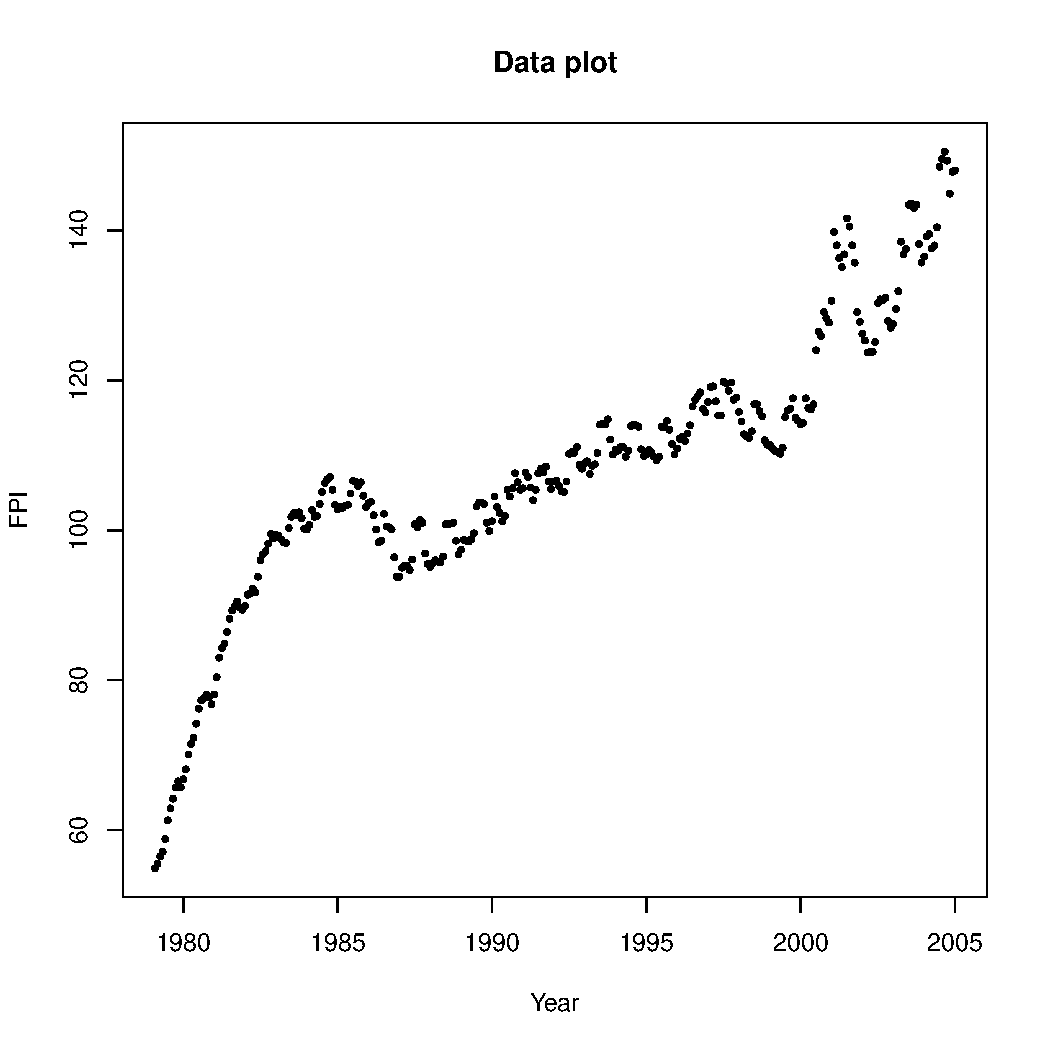
\includegraphics[width=100mm]{data-plot.pdf}
    \caption{Plot of fuel price index as function of time}
    \label{fig:plot-question-1}
\end{figure}

To get an overview of the data the fuel price index is plotted as a function of time and the resulting plot is shown in figure~\ref{fig:plot-question-1}. From the plot it is seen that the \fpi\ grew rapidly from 1979 to 1985 and with small variation between months (the points almost follows a straight line). After a period with decrease between 1985-1987 a long period (1987-1997) with slow increase follows. The variation between months is larger than for the 1979-1985 period. From 2000 to mid-2001 the \fpi\ increases rapidly followed by a short decrease from mid-2001 to start-2002. From start-2002 to the end of 2004 the \fpi\ once more grows fast and the variation between months is larger than for any of the previous periods. \\

From the description of the data it should be clear that it won't make much sense to estimate a global mean and standard deviation from the data as the \fpi\ don't seem to vary around a mean value but rather to steadily increase, only interrupted by short periods of decrease. We therefore have to rule out the constant mean model\footnote{See equation $3.63$ in \cite{hm}} and will instead start out by fitting a global linear model to the data.

\section*{General linear model}
As an first attempt to make predictions it is assumed that the \fpi\ can be modeled as a first order polynomial of time with some white noise added. The white noise represents the various random phenomenom that influences the \fpi. The model is
\begin{equation*}
    Y_t = \theta_0 + \theta_1 t + \varepsilon_t
\end{equation*}
where $\varepsilon_t$ is assumed to be i.i.d random variables with $\E{\varepsilon_t}=0$ and $\Var{\varepsilon_t}=\sigma^2$. Using R the model parameters are estimated from the data and gives 
\begin{equation*}
    Y_t = -4198 + 2.162 t + \varepsilon_t
\end{equation*}
A plot of the model is shown in figure~\ref{fig:fitted-linear-model}. From the plot it is seen that the model do not fit the data very well. For the early data points the model predictions are too high and for the data points near 2005 the model seems to predict lower than the observed \fpi. The poor fit of the model can be further illustrated by plotting the residuals $\varepsilon_t$. If the model fitted the data well the residuals would be pure white noise and no structure would be seen in the residuals plot. But as seen in figure~\ref{fig:fitted-linear-model-residuals} a lot of structure remains in the residuals and the conclusion is that the simple linear model is not appropriate for making predictions.

\begin{figure}
    \centering
    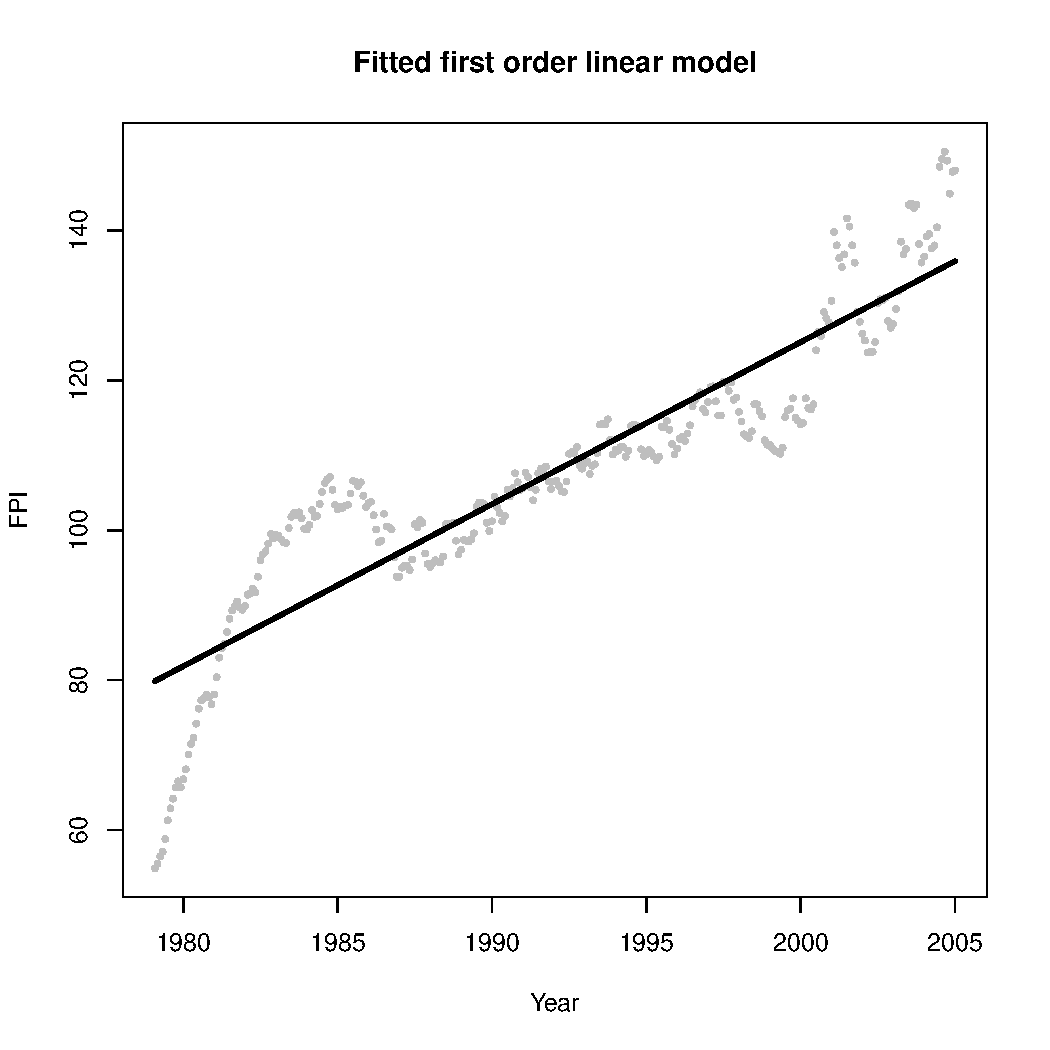
\includegraphics[width=100mm]{fitted-linear-model.pdf}
    \caption{Plot of simple linear model}
    \label{fig:fitted-linear-model}
\end{figure}

\begin{figure}
    \centering
    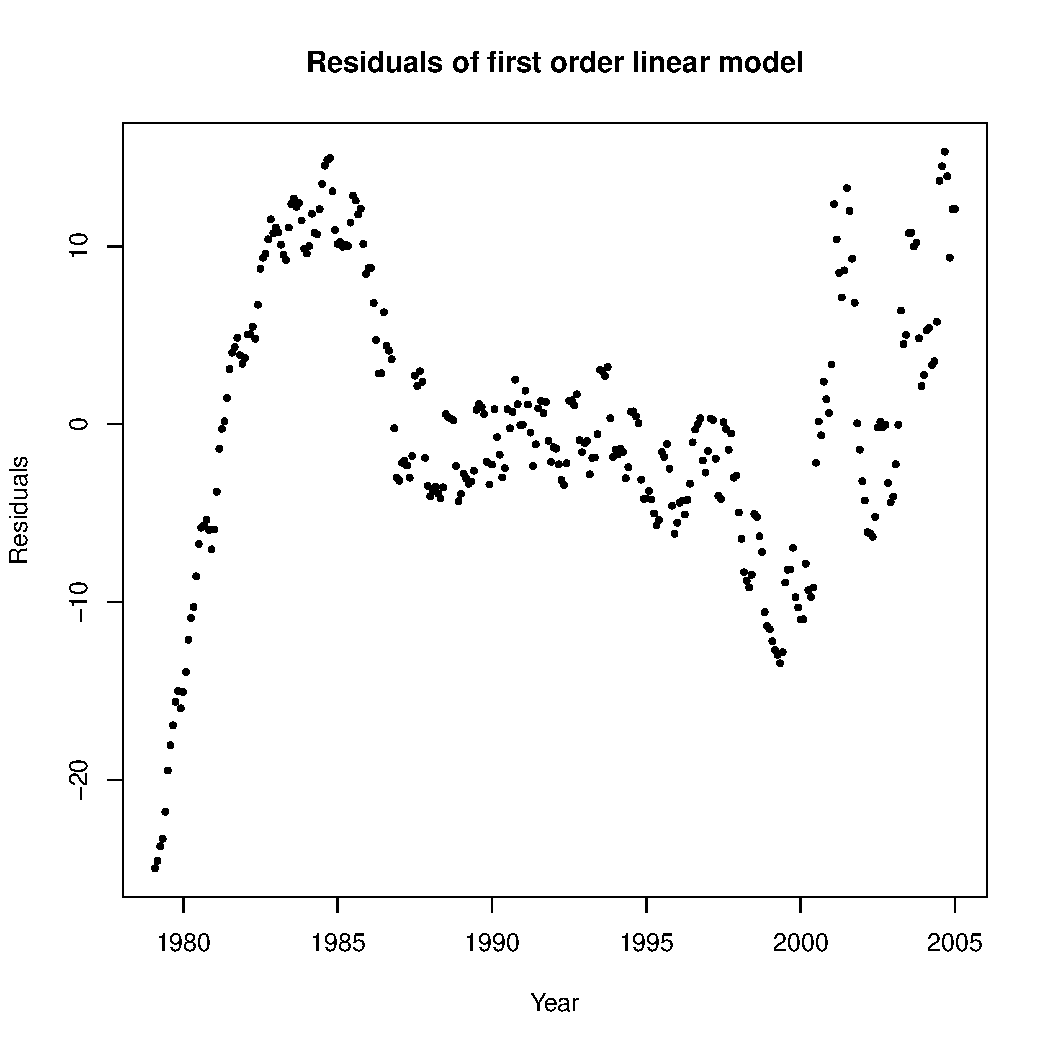
\includegraphics[width=100mm]{fitted-linear-model-residuals.pdf}
    \caption{Plot of residuals for the simple linear model}
    \label{fig:fitted-linear-model-residuals}
\end{figure}


\section*{Local constant mean model}
One of the problems with the simple linear regression used in the previous section is that it tries to fit all the data. This means that the measured \fpi\ in 1979 influences the predictions for 2005 as much as the measured \fpi\ in December 2004. To counteract this we now use a local constant mean model. In this model the mean of \fpi\ is allowed to change by giving more weight to the most recent observations (see \cite[p. 50]{hm}). In theory all previous observations still influences predictions, but in practice only the few most recent observations are important. How many observations that influences the prediction can be controlled by changing the forgetting factor $\lambda$. \par
To predict the \fpi\ for the first half of 2005 a local constant mean model was created for $\lambda=0.2$ and $\lambda=0.8$. The results are shown in figure~\ref{fig:local-constant-2} and figure~\ref{fig:local-constant-8}. For $\lambda=0.2$ all predictions are almost identical and almost equal to the newest observation of \fpi. For $\lambda=0.8$ the predictions start out a bit lower but converges toward the value of the newest observation\footnote{Actually I don't quite get this result. In equation $3.70$ in the course textbook, it is stated that all future prediction, given a data set, should be equal. Using equation 3.75 I get predictions that are not exactly equal. Am I doing something wrong?}.


\begin{figure}
    \centering
    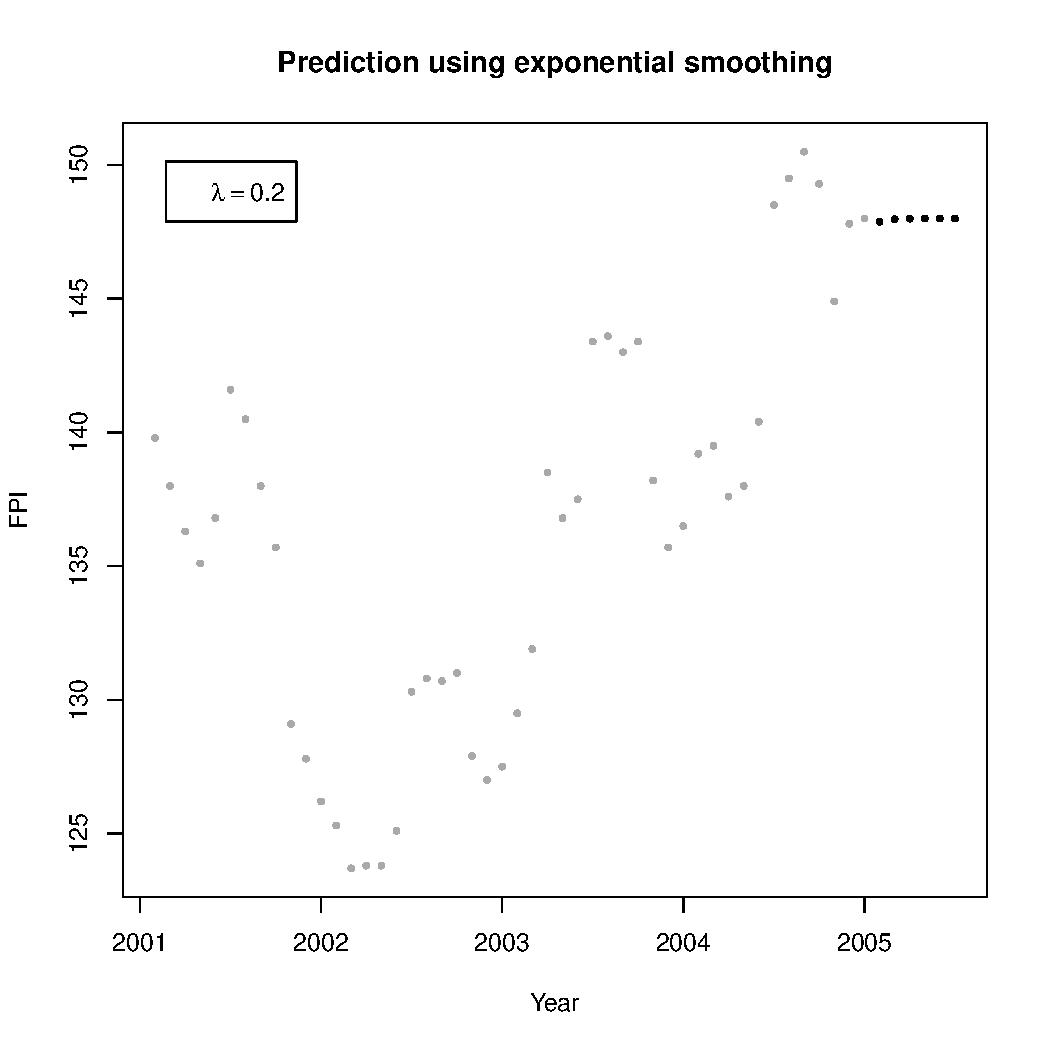
\includegraphics[width=100mm]{exp-smoothing-lambda-2.pdf}
    \caption{Plot of simple linear model}
    \label{fig:local-constant-2}
\end{figure}

\begin{figure}
    \centering
    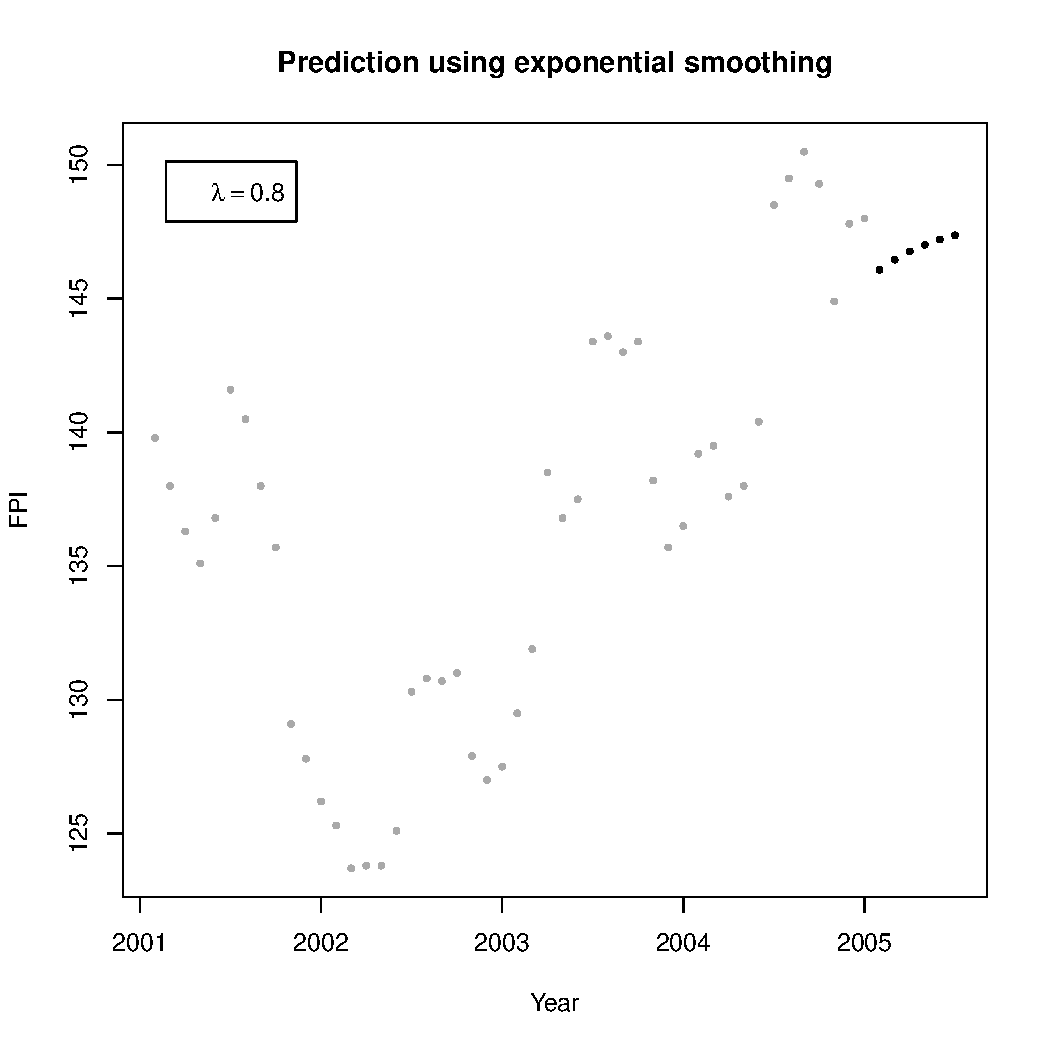
\includegraphics[width=100mm]{exp-smoothing-lambda-8.pdf}
    \caption{Plot of simple linear model}
    \label{fig:local-constant-8}
\end{figure}

\pagebreak

\section*{Local trend model}
In the previous section the predictions was improved, compared to the simple linear model, by giving more weight to the most recent observation. But the model was simple and the predictions were almost equal which doesn't seem plausible. In this section a model that is linear in time and that gives most weight to the most recent observations is utilized. The model is called a local trend model and is just a special kind of WLS model where the weights are chosen as powers of the forgetting factor $\lambda$. Predictions and confidence intervals for the predictions is calculated (with $\lambda=0.6$) and the result is shown in figure~\ref{fig:local-trend-model-normal}. It can be seen that the prediction for January 2005 is again very close to the value of December 2004, but unlike the previous model, predictions for the other months of 2005 are now linearly increasing. 

\begin{figure}
    \centering
    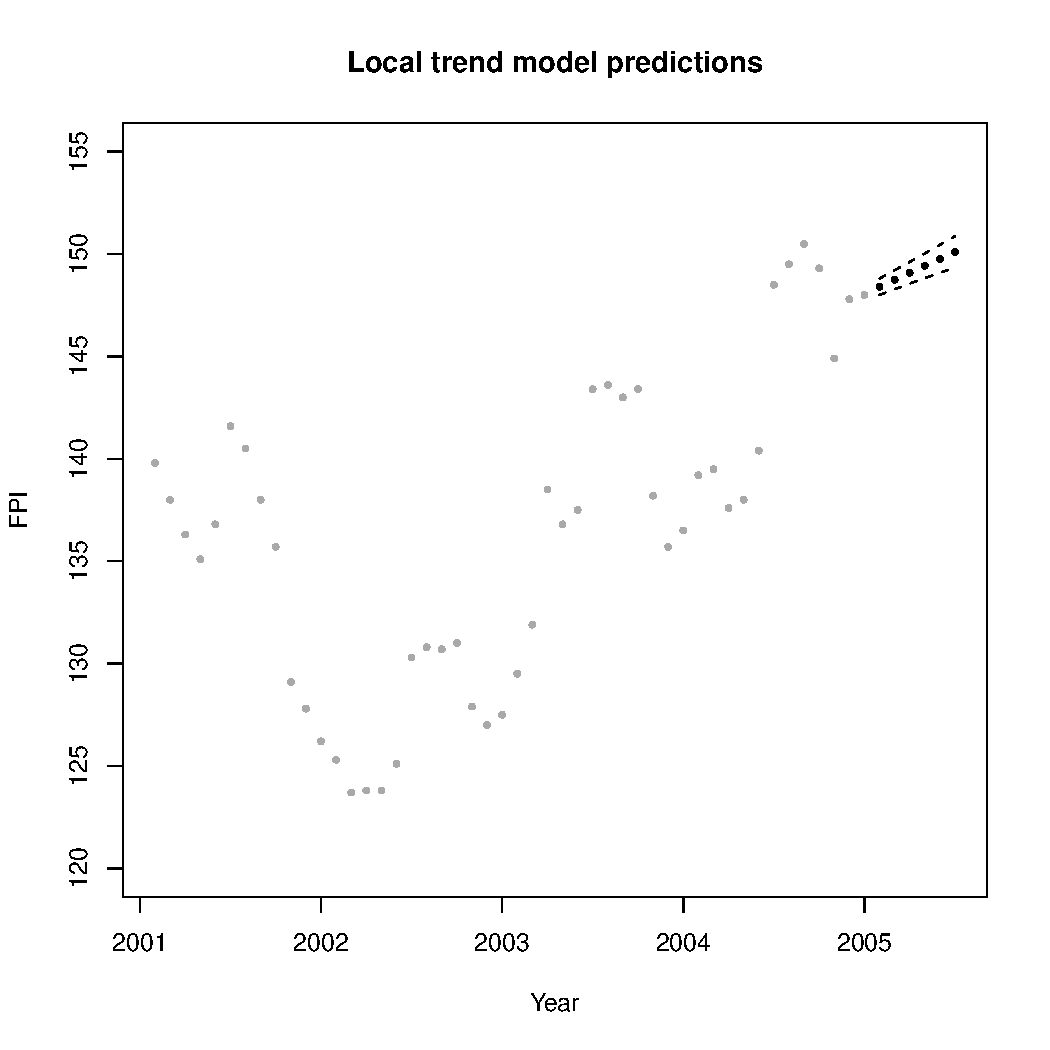
\includegraphics[width=100mm]{local-trend-predict-normal-6.pdf}
    \caption{Plot of simple linear model}
    \label{fig:local-trend-model-normal}
\end{figure}

\subsection*{Calculating the confidence intervals}
The confidence intervals for the predictions seems very optimistic but this could be due to the fact that the covariance matrix $\mathbf{\Sigma}$ is very ill-conditioned. From a computational point of view the covariance matrix is singular which means that $\mathbf{\Sigma^{-1}}$ can't be calculated directly and therefore equation 3.44 in \cite{hm} can't be used to calculate $\widehat{\sigma}^2$. Instead $\widehat{\sigma}^2$ was calculated by (using the notation from \cite{hm})
\begin{gather*}
    S(\widehat{\boldsymbol{\theta}}) = \sum_{j=0}^{N-1} \lambda^j(Y_{N-j} - \boldsymbol{f}^T(-j)\widehat{\boldsymbol{\theta}}_N) \\
    \widehat{\sigma}^2 = \frac{S(\widehat{\boldsymbol{\theta}})}{N-p}
\end{gather*}
The problem with this approach is that for most values of $j$, $\lambda^j$ is smaller than machine precision and therefore only a small number of the $N$ observations are included in the calculation. But from the formula above it is seen that we still divide by $N-p$ so $\widehat{\sigma}^2$ becomes smaller than it should be. A pragmatic solution is to count for how many $j$'s $\lambda^j$ is above some threshold (e.g. $10^{-6}$) and then use this number instead of $N$. This was implemented and a new set of confidence intervals was calculated. The result is shown in figure~\ref{fig:local-trend-model-adjusted} and now the confidence interval seems much more plausible.

\begin{figure}
    \centering
    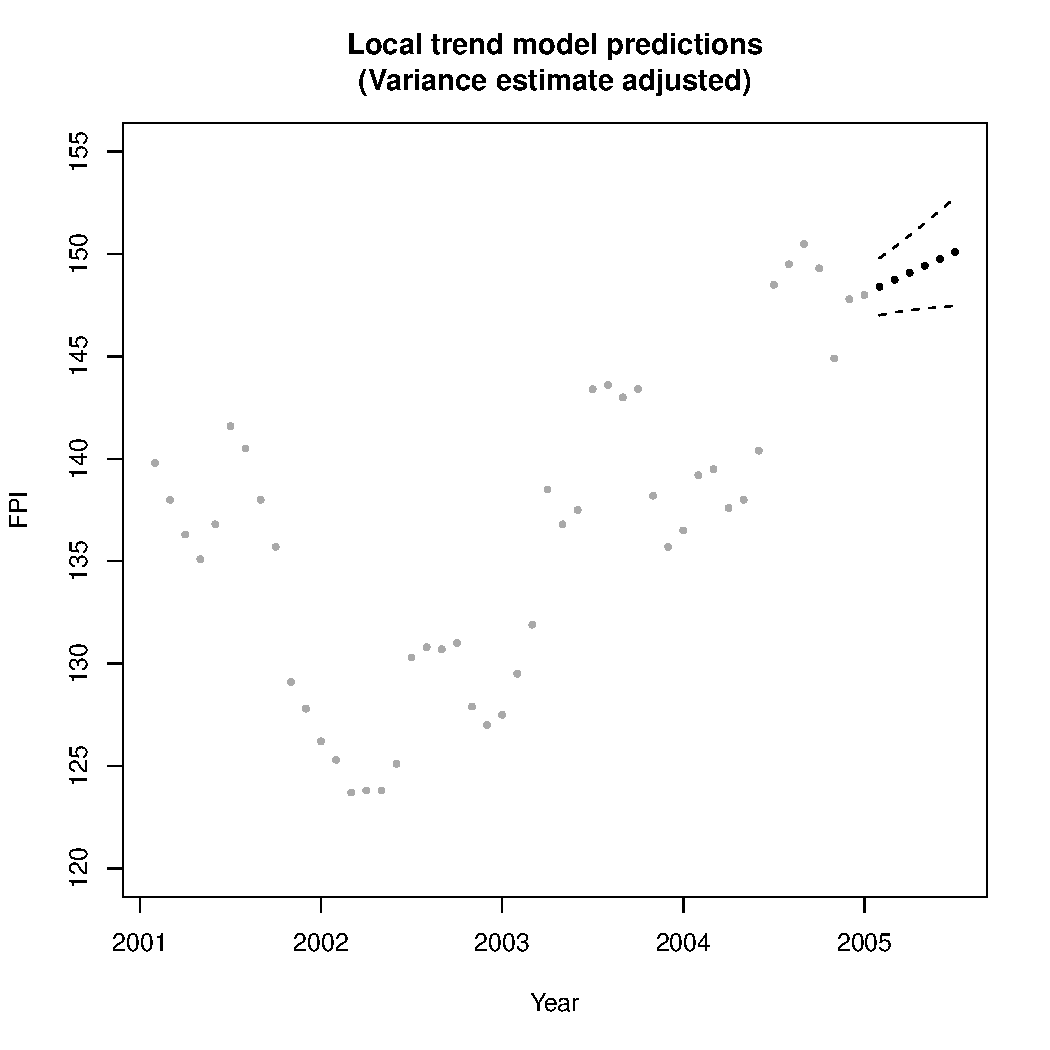
\includegraphics[width=100mm]{local-trend-predict-adjusted-6.pdf}
    \caption{Plot of simple linear model}
    \label{fig:local-trend-model-adjusted}
\end{figure}


\subsection*{Selecting $\lambda$}
The model seems to be useful but in the previous subsection $\lambda$ was randomly chosen as 0.6. It now needs to be determined what value of $\lambda$ fits the data best. Therefore the one-step prediction errors (see eq. 3.78 and 3.79 in \cite{hm}) are calculated for various lambda values and the result is shown in figure~\ref{fig:prediction-errors}.

\begin{figure}
    \centering
    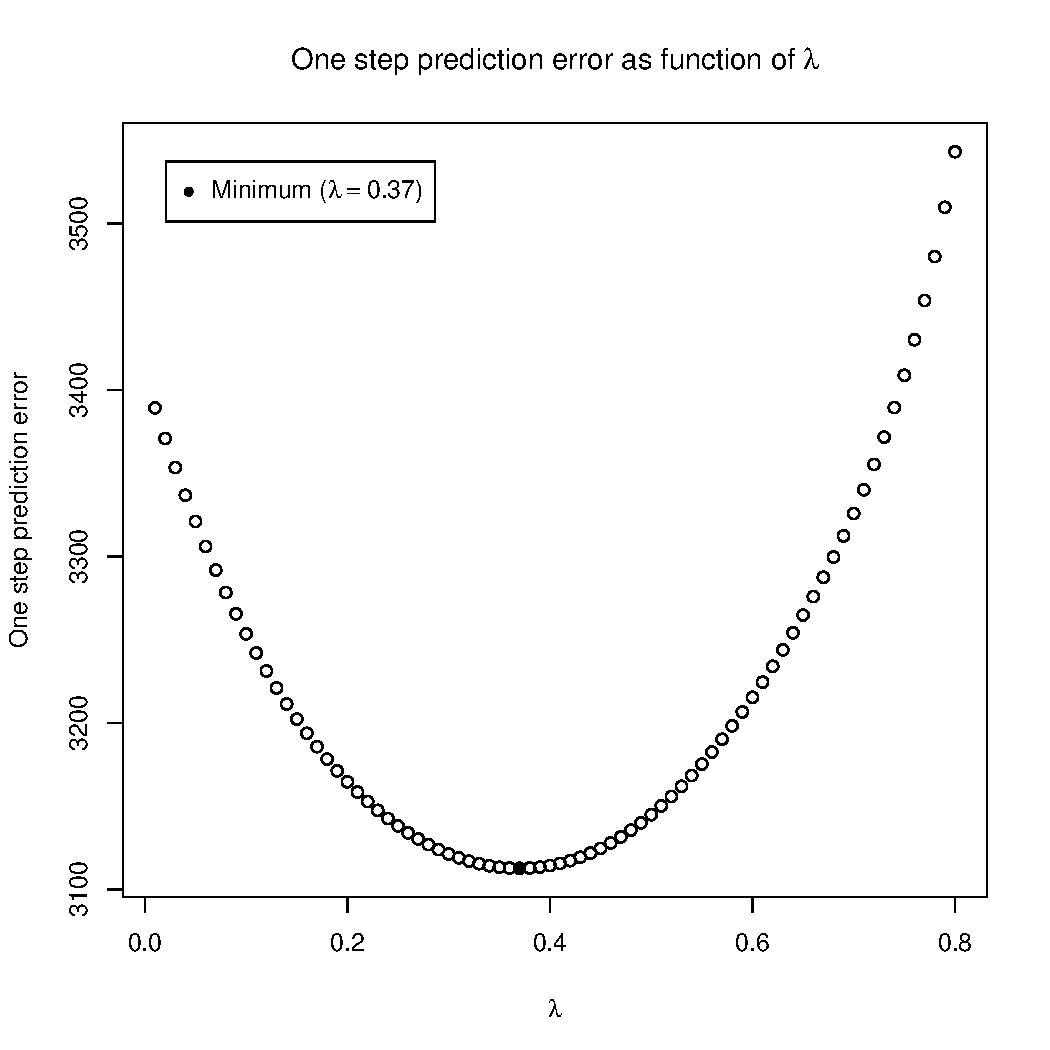
\includegraphics[width=100mm]{prediction-errors.pdf}
    \caption{Plot of simple linear model}
    \label{fig:prediction-errors}
\end{figure}

\subsection*{Final model}
The local trend model is now estimated for $\lambda=0.37$ and predictions and confidence intervals are calculated. The result is shown in figure~\ref{fig:trend-model-adjusted-37}

\begin{figure}
    \centering
    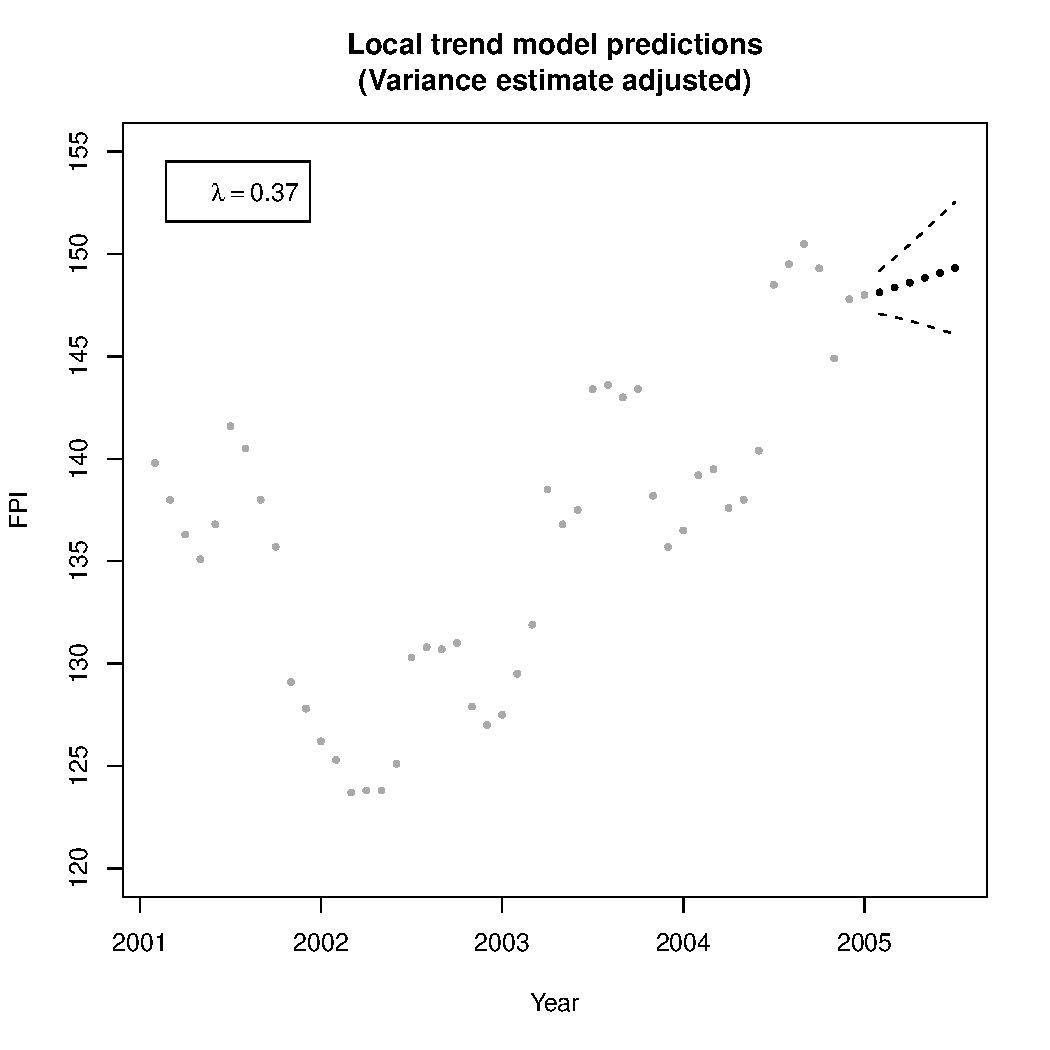
\includegraphics[width=100mm]{local-trend-predict-adjusted-37.pdf}
    \caption{Plot of simple linear model}
    \label{fig:local-trend-model-adjusted-37}
\end{figure}


\pagebreak

\section*{Appendices}
All R code used for this assignment are included here. All source code incl. latex code for this report can be found at \url{http://github.com/alphabits/dtu-fall-2011/}
\subsection*{Loading data (loaddata.R)}
\lstinputlisting{loaddata.R}
\subsection*{Data plot (ex-1.R)}
\lstinputlisting{ex-1.R}
\subsection*{Simple linear model (ex-3.R)}
\lstinputlisting{ex-3.R}
\subsection*{Exponential smoothing (ex-4.R)}
\lstinputlisting{ex-4.R}
\subsection*{Local trend model (ex-5.R)}
\lstinputlisting{ex-5.R}
\subsection*{Determine optimal $\lambda$ (ex-6.R)}
\lstinputlisting{ex-6.R}
\subsection*{Functions for local trend model (local-trend-functions.R)}
\lstinputlisting{local-trend-functions.R}


\pagebreak

\begin{thebibliography}{9}

\bibitem{hm}
  Henrik Madsen,
  \emph{Time Series Analysis}.
  Chapman \& Hall/CRC,
  1st Edition,
  2008.

\end{thebibliography}
\end{document}
